\documentclass[12pt,letterpaper]{article}

% ---------- paquetes ----------
\usepackage[utf8]{inputenc}
\usepackage[T1]{fontenc}
\usepackage[spanish]{babel}
\usepackage{times}
\usepackage[margin=2.54cm, headheight=15pt]{geometry}
\usepackage{setspace}
\usepackage{graphicx}
\usepackage{float}
\usepackage{booktabs}
\usepackage{array}
\usepackage{longtable}
\usepackage{xcolor}
\usepackage{hyperref}
\usepackage{url}
\usepackage{fancyhdr}
\usepackage{titlesec}
\usepackage{parskip}
\usepackage{caption}
\usepackage{listings}
\usepackage{microtype}

% ---------- colores y estilo código ----------
\definecolor{codegreen}{rgb}{0,0.5,0}
\definecolor{codegray}{rgb}{0.5,0.5,0.5}
\definecolor{backcolor}{rgb}{0.97,0.97,0.97}

\lstdefinestyle{bashstyle}{
  backgroundcolor=\color{backcolor},
  commentstyle=\color{codegreen},
  keywordstyle=\color{blue},
  basicstyle=\ttfamily\small,
  breakatwhitespace=false,
  breaklines=true,
  captionpos=b,
  frame=single,
  keepspaces=true,
  showspaces=false,
  showstringspaces=false,
  tabsize=2,
  language=bash
}

% ---------- interlineado APA ----------
\doublespacing

% ---------- encabezado / pie ----------
\pagestyle{fancy}
\fancyhf{}
\fancyhead[R]{\thepage}
\fancyhead[L]{\small Hardening con OpenSCAP en Ubuntu Server 24.04}
\renewcommand{\headrulewidth}{0pt}

% ---------- hiperenlaces ----------
\hypersetup{
  colorlinks=true,
  linkcolor=black,
  citecolor=black,
  urlcolor=blue
}

% ---------- sin sangría, espacio entre párrafos ----------
\setlength{\parindent}{0.5in}
\setlength{\parskip}{0pt}

\begin{document}

% ============================================================
%  PORTADA
% ============================================================
\begin{titlepage}
  \centering
  \vspace*{1cm}

  {\large\bfseries Universidad Tecnológica del Perú}\\[0.3cm]
  {\large Especialización en Tecnologías de la Información y Comunicación}\\[0.2cm]
  {\large Curso: Ciberseguridad}\\[3cm]

  {\LARGE\bfseries Actividad \#3}\\[0.5cm]
  {\Large Hardening de Ubuntu Server 24.04 con OpenSCAP\\
  y SCAP Security Guide}\\[3cm]

  \begin{flushleft}
    {\large\bfseries Estudiante:}\\[0.2cm]
    {\large Daniel Toro Soto}\\[1cm]
    {\large\bfseries Docente:}\\[0.2cm]
    {\large Camilo Cadavid}\\[1cm]
    {\large\bfseries Fecha de entrega:}\\[0.2cm]
    {\large 6 de junio de 2026}
  \end{flushleft}

  \vfill
\end{titlepage}

% ============================================================
%  TABLA DE CONTENIDO
% ============================================================
\tableofcontents
\newpage

% ============================================================
%  1. INTRODUCCIÓN
% ============================================================
\section{Introducción}

En el panorama actual de la ciberseguridad, los sistemas operativos recién instalados presentan configuraciones predeterminadas que priorizan la usabilidad sobre la seguridad. Este estado, conocido como configuración \textit{out-of-the-box}, expone a los servidores a una amplia superficie de ataque que puede ser explotada por actores maliciosos. El \textit{hardening} —o endurecimiento— es el proceso sistemático de reducir dicha superficie mediante la aplicación de controles de seguridad que limitan las vías de ataque sin comprometer la funcionalidad del sistema.

El hardening abarca diversas áreas: configuración de SSH, auditoría del sistema, gestión de permisos de archivos, restricción de módulos del kernel innecesarios, aplicación de políticas de contraseñas robustas, y deshabilitación de servicios no requeridos, entre otros. Aplicar estas medidas de forma manual es propenso a errores y difícilmente reproducible; por ello, existen frameworks estandarizados como el \textit{Security Content Automation Protocol} (SCAP) que automatizan tanto la evaluación como la remediación.

La presente actividad tiene como objetivo aplicar un proceso de hardening completo sobre una instalación limpia de Ubuntu Server 24.04, utilizando las herramientas OpenSCAP y la SCAP Security Guide bajo el perfil CIS Level 1 para servidores. Se documentan los pasos seguidos, se comparan los resultados antes y después de las remediaciones, y se analiza la mejora obtenida en la postura de seguridad del sistema.

% ============================================================
%  2. MARCO TEÓRICO
% ============================================================
\section{Marco Teórico}

\subsection{Hardening de sistemas operativos}

El hardening es el conjunto de prácticas destinadas a reducir la vulnerabilidad de un sistema informático mediante la eliminación de vectores de ataque innecesarios (Center for Internet Security [CIS], 2024). Incluye la desactivación de servicios no esenciales, la configuración segura de los servicios activos, la aplicación de actualizaciones de seguridad y el establecimiento de controles de acceso estrictos. El objetivo no es crear un sistema inexpugnable —lo cual es inalcanzable en la práctica— sino aumentar el costo de un ataque hasta el punto en que resulte impráctico para la mayoría de los adversarios.

\subsection{SCAP (Security Content Automation Protocol)}

El \textit{Security Content Automation Protocol} es un conjunto de estándares abiertos promovido por el Instituto Nacional de Estándares y Tecnología (NIST) que permite la automatización de la gestión de vulnerabilidades, la medición y la evaluación del cumplimiento de políticas de seguridad (National Institute of Standards and Technology [NIST], 2011). SCAP integra varios componentes:

\begin{itemize}
  \item \textbf{XCCDF} (\textit{Extensible Configuration Checklist Description Format}): lenguaje XML para describir listas de comprobación de seguridad y sus resultados.
  \item \textbf{OVAL} (\textit{Open Vulnerability and Assessment Language}): lenguaje para representar información sobre el estado de un sistema y si cumple o no ciertos criterios.
  \item \textbf{CPE} (\textit{Common Platform Enumeration}): esquema de nomenclatura para plataformas de TI.
  \item \textbf{CVE} (\textit{Common Vulnerabilities and Exposures}): identificadores estándar para vulnerabilidades conocidas.
\end{itemize}

\subsection{OpenSCAP}

OpenSCAP es la implementación de código abierto del estándar SCAP, desarrollada principalmente por Red Hat y la comunidad de software libre (OpenSCAP, 2024). Proporciona un motor de evaluación (\texttt{oscap}) capaz de leer políticas SCAP y ejecutarlas sobre el sistema operativo local, generando informes en formato HTML y XML con los resultados de cada control. Entre sus funcionalidades destacan:

\begin{itemize}
  \item Evaluación (\texttt{oscap xccdf eval}): comprueba el estado del sistema contra un perfil de seguridad.
  \item Remediación automática (\texttt{--remediate}): aplica los cambios necesarios para corregir los controles fallidos.
  \item Generación de scripts de remediación: produce scripts Bash o playbooks Ansible con todas las correcciones.
  \item Generación de informes HTML interactivos: permite visualizar en un navegador el estado de cada control.
\end{itemize}

\subsection{CIS Benchmarks}

El \textit{Center for Internet Security} publica los CIS Benchmarks, guías de buenas prácticas de configuración segura para sistemas operativos, middleware y aplicaciones (CIS, 2024). Estas guías se articulan en dos niveles:

\begin{itemize}
  \item \textbf{Level 1}: conjunto de controles básicos con bajo impacto operativo, aplicables en la mayoría de entornos.
  \item \textbf{Level 2}: controles adicionales más restrictivos, orientados a entornos de alta seguridad.
\end{itemize}

Para esta actividad se utilizó el perfil CIS Level 1 para servidores (\texttt{cis\_level1\_server}), que ofrece una base sólida de seguridad sin comprometer la operatividad del sistema.

\subsection{SCAP Security Guide (SSG)}

La \textit{SCAP Security Guide} es un proyecto de ComplianceAsCode que traduce los CIS Benchmarks y otras políticas de seguridad (STIG, PCI-DSS, etc.) al formato SCAP, haciéndolas consumibles por herramientas como OpenSCAP (ComplianceAsCode, 2024). El archivo principal para Ubuntu 24.04, \texttt{ssg-ubuntu2404-ds.xml}, fue introducido a partir de la versión 0.1.76 del proyecto.

% ============================================================
%  3. METODOLOGÍA
% ============================================================
\section{Metodología}

La actividad se llevó a cabo en un entorno virtualizado utilizando UTM sobre un Mac Mini M4. Ubuntu Server 24.04 (ARM64) se instaló como máquina virtual con 2 núcleos de CPU, 2 GB de RAM y 20 GB de almacenamiento.

\subsection{Fase 1: Instalación de Ubuntu Server 24.04}

Se creó una máquina virtual en UTM seleccionando la opción \textit{Virtualize → Linux} y el ISO de Ubuntu Server 24.04 (ARM64). Durante la instalación se habilitó el servidor OpenSSH para facilitar el acceso remoto desde el Mac anfitrión.

\begin{figure}[H]
  \centering
  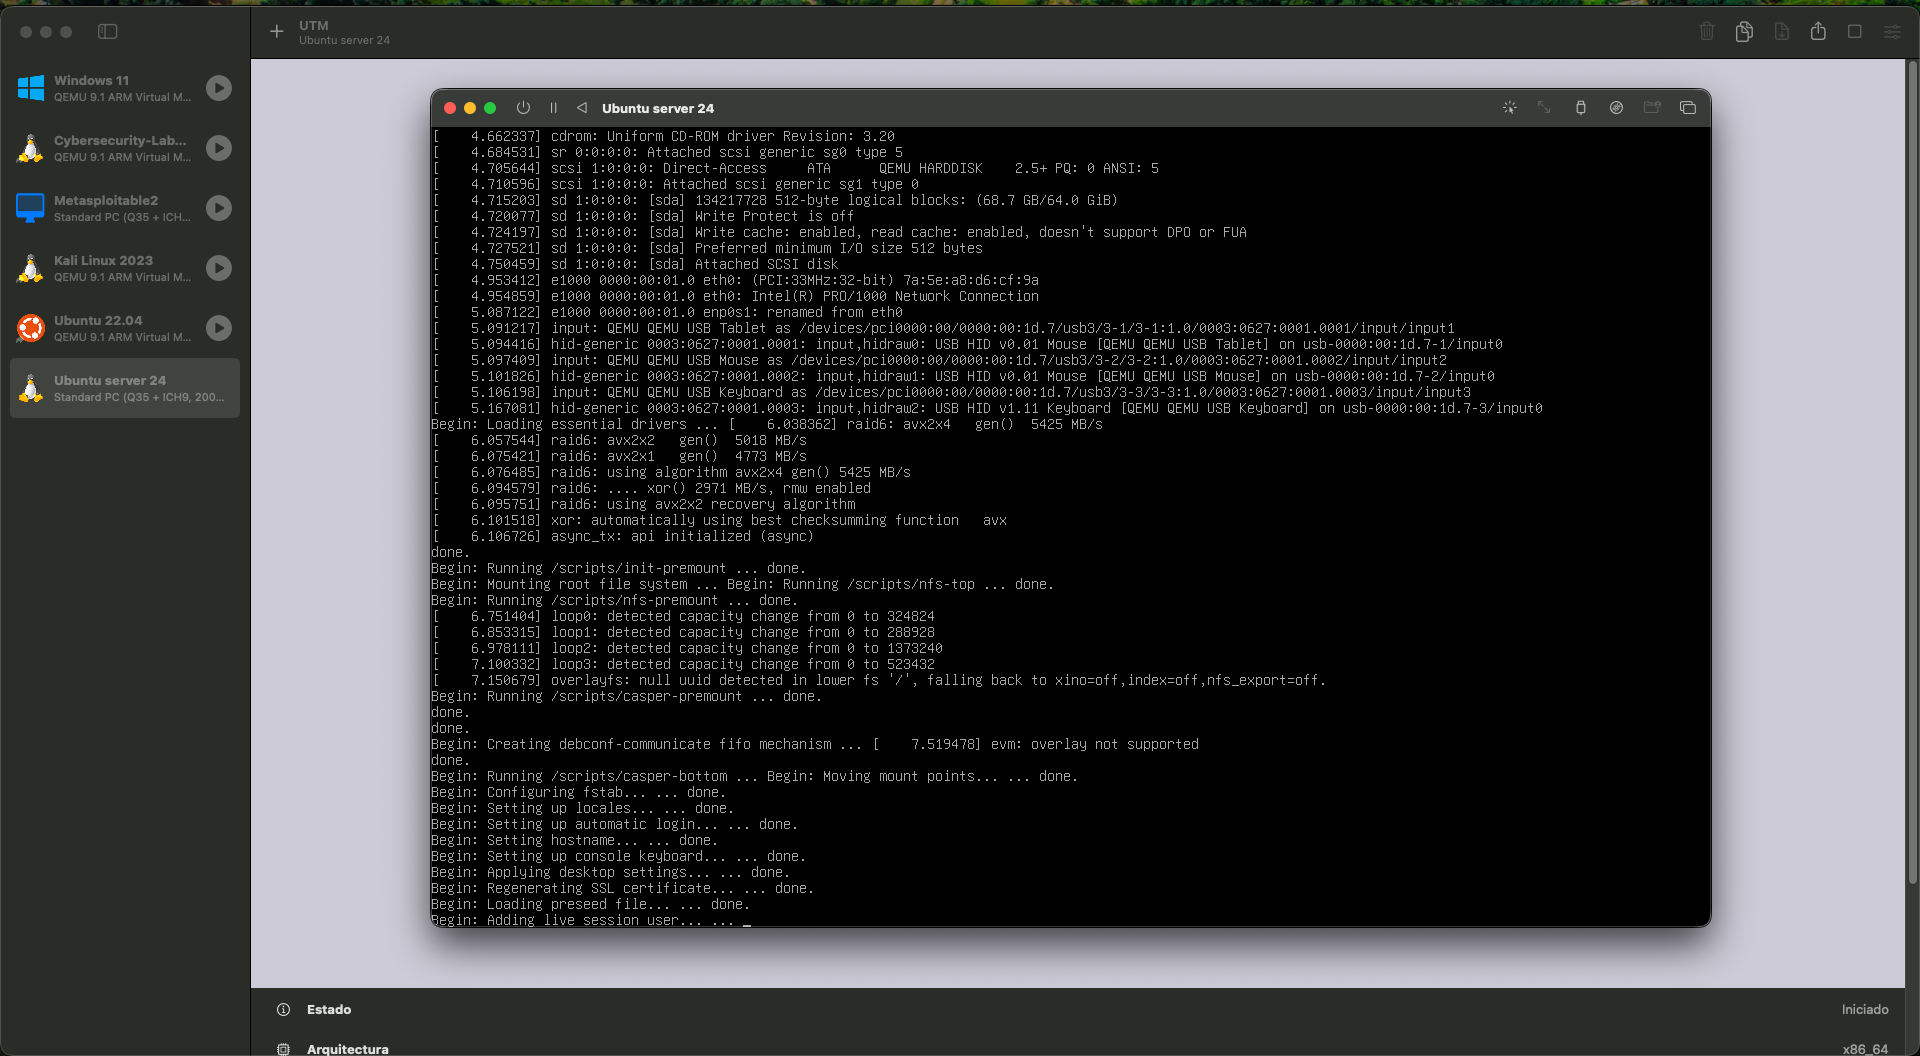
\includegraphics[width=0.85\textwidth]{../img/installing_ubuntu_server.png}
  \caption{Proceso de instalación de Ubuntu Server 24.04 en UTM.}
  \label{fig:instalacion}
\end{figure}

\begin{figure}[H]
  \centering
  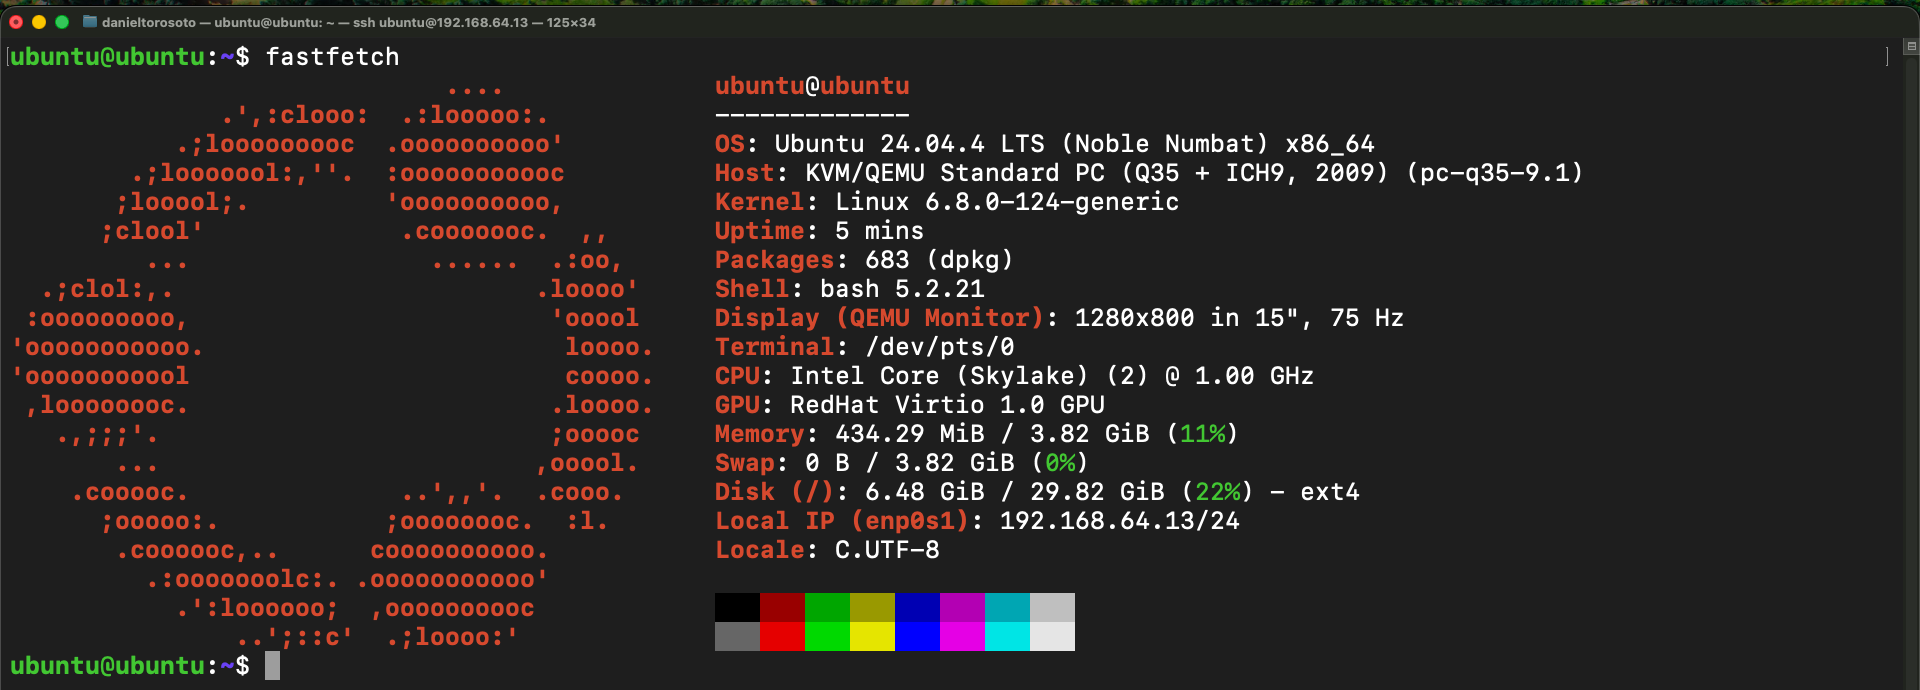
\includegraphics[width=0.85\textwidth]{../img/ssh_from_mac_showing_fastfetch.png}
  \caption{Acceso SSH exitoso desde el Mac anfitrión a la VM Ubuntu Server 24.04.}
  \label{fig:ssh}
\end{figure}

\subsection{Fase 2: Instalación de OpenSCAP}

Una vez dentro de la VM, se instaló el escáner OpenSCAP desde los repositorios oficiales de Ubuntu:

\begin{lstlisting}[style=bashstyle, caption={Instalación de OpenSCAP en Ubuntu Server 24.04}]
sudo apt update && sudo apt upgrade -y
sudo apt install -y openscap-scanner openscap-common
oscap --version
\end{lstlisting}

\textit{Nota:} En Ubuntu 24.04 el paquete fue renombrado de \texttt{libopenscap8} a \texttt{openscap-common} y \texttt{libopenscap25t64}; se utilizó la denominación correcta para esta versión.

\begin{figure}[H]
  \centering
  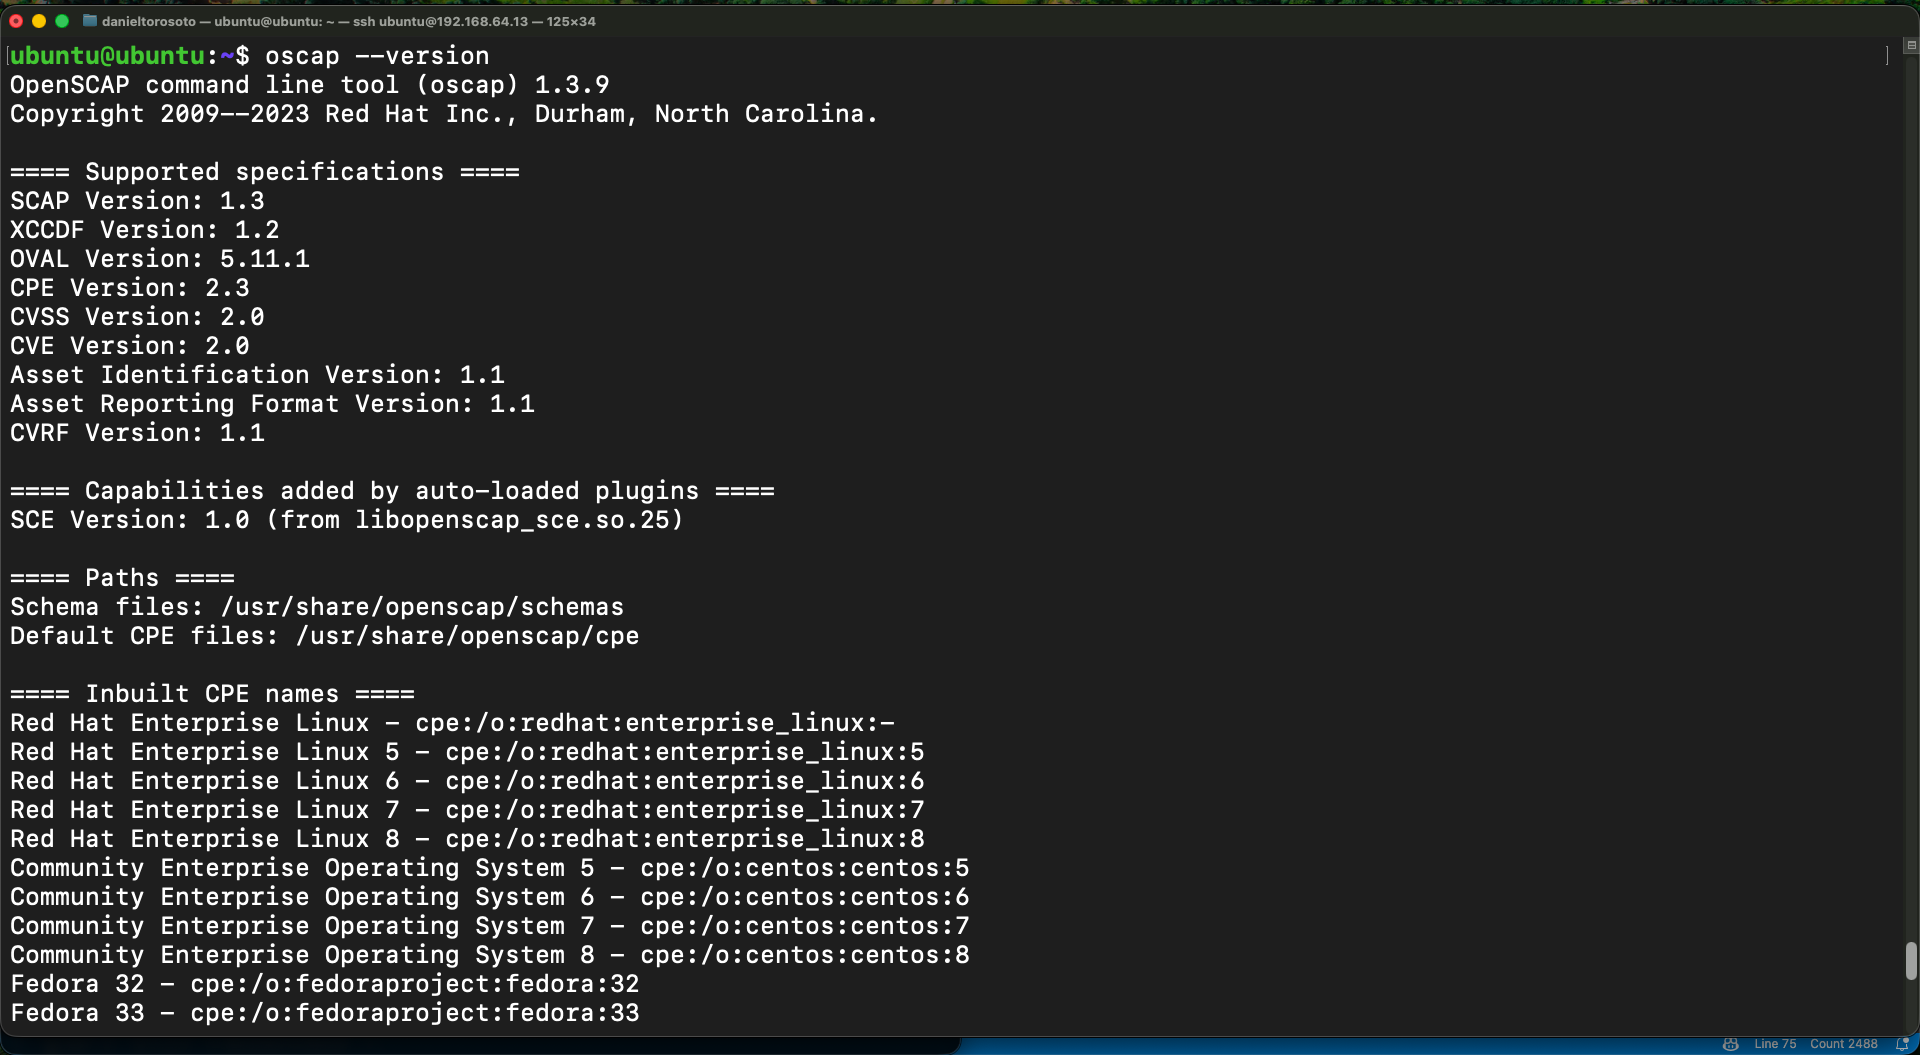
\includegraphics[width=0.85\textwidth]{../img/ssh_oscap_installed.png}
  \caption{OpenSCAP instalado y verificado con \texttt{oscap --version}.}
  \label{fig:oscap-instalado}
\end{figure}

\subsection{Fase 3: Descarga de la SCAP Security Guide}

Los paquetes \texttt{ssg-base} y \texttt{ssg-debderived} disponibles en los repositorios de Ubuntu 24.04 no incluían aún el archivo para Ubuntu 24.04 (\texttt{ssg-ubuntu2404-ds.xml}). Se descargó la versión 0.1.76 del proyecto ComplianceAsCode directamente desde GitHub, primera versión que incorpora soporte para Ubuntu 24.04:

\begin{lstlisting}[style=bashstyle, caption={Descarga de la SCAP Security Guide v0.1.76}]
wget https://github.com/ComplianceAsCode/content/releases/\
  download/v0.1.76/scap-security-guide-0.1.76.zip
sudo apt install -y unzip
unzip scap-security-guide-0.1.76.zip
ls ~/scap-security-guide-0.1.76/ssg-ubuntu2404-ds.xml
\end{lstlisting}

\begin{figure}[H]
  \centering
  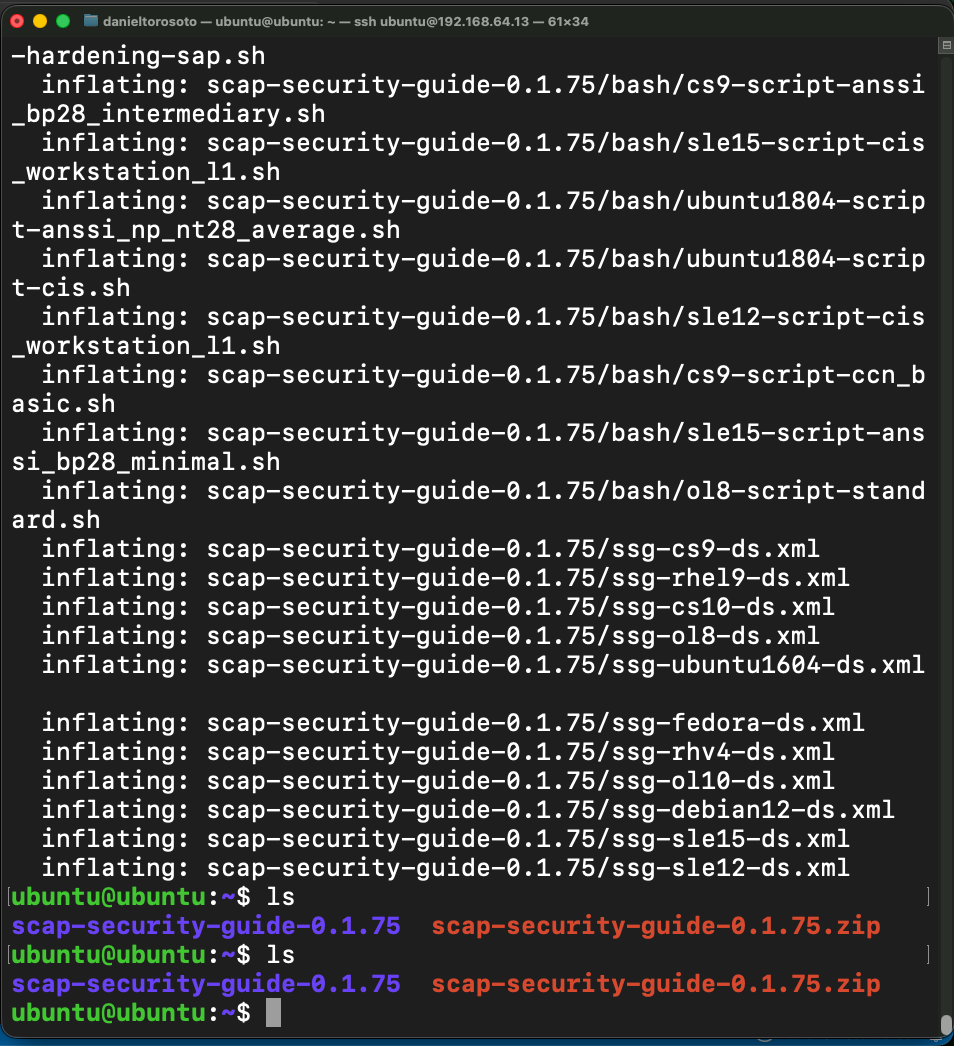
\includegraphics[width=0.85\textwidth]{../img/ssh_scap_security_guide.png}
  \caption{Archivo de política \texttt{ssg-ubuntu2404-ds.xml} disponible tras descomprimir la SSG v0.1.76.}
  \label{fig:ssg}
\end{figure}

\subsection{Fase 4: Escaneo inicial (línea base)}

Se definió la variable de entorno \texttt{SSG} con la ruta al archivo de política y se ejecutó la evaluación con el perfil CIS Level 1 para servidores:

\begin{lstlisting}[style=bashstyle, caption={Escaneo inicial con el perfil CIS Level 1 Server}]
SSG="$HOME/scap-security-guide-0.1.76/ssg-ubuntu2404-ds.xml"

sudo oscap xccdf eval \
  --profile xccdf_org.ssgproject.content_profile_cis_level1_server \
  --results /tmp/resultado-inicial.xml \
  --report /tmp/reporte-inicial.html \
  "$SSG"
\end{lstlisting}

\begin{figure}[H]
  \centering
  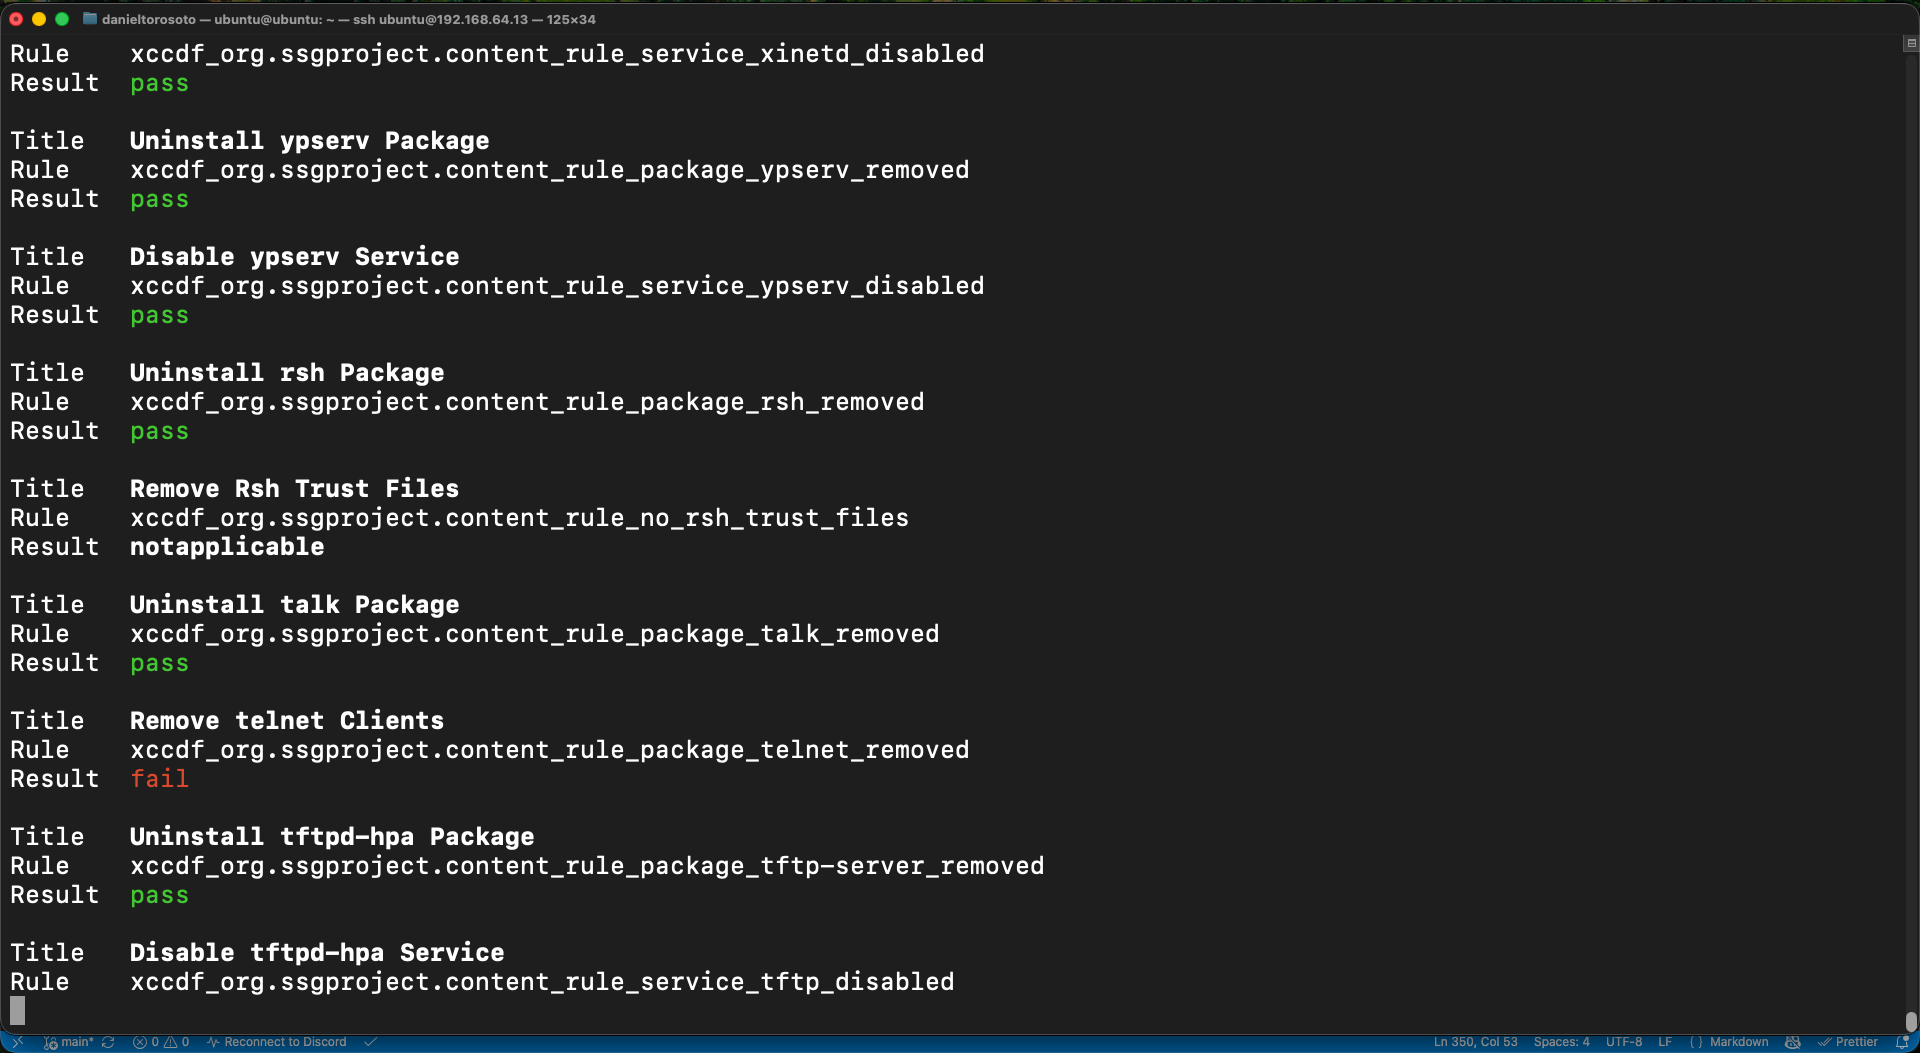
\includegraphics[width=0.85\textwidth]{../img/running_initial_scan.png}
  \caption{Ejecución del escaneo inicial en la terminal de la VM.}
  \label{fig:escaneo-inicial}
\end{figure}

\subsection{Fase 5: Remediación automática}

Antes de aplicar las remediaciones, se creó un snapshot de la VM en UTM como medida de seguridad. Acto seguido, se ejecutó OpenSCAP en modo de remediación integrada, el cual evalúa cada control y aplica de inmediato los cambios necesarios cuando el control falla:

\begin{lstlisting}[style=bashstyle, caption={Remediación automática con OpenSCAP}]
SSG="$HOME/scap-security-guide-0.1.76/ssg-ubuntu2404-ds.xml"

sudo oscap xccdf eval \
  --remediate \
  --profile xccdf_org.ssgproject.content_profile_cis_level1_server \
  --results /tmp/resultado-post-remediation.xml \
  --report /tmp/reporte-post-remediation.html \
  "$SSG"

sudo reboot
\end{lstlisting}

El proceso de remediación abarcó controles relacionados con: configuración de SSH, auditoría del sistema (\texttt{auditd}), permisos de archivos críticos, restricción de módulos del kernel innecesarios (USB storage, Bluetooth, firewire), políticas de contraseñas, configuración del firewall (\texttt{ufw}), y desactivación de servicios no requeridos. El proceso tardó aproximadamente 30 minutos.

\begin{figure}[H]
  \centering
  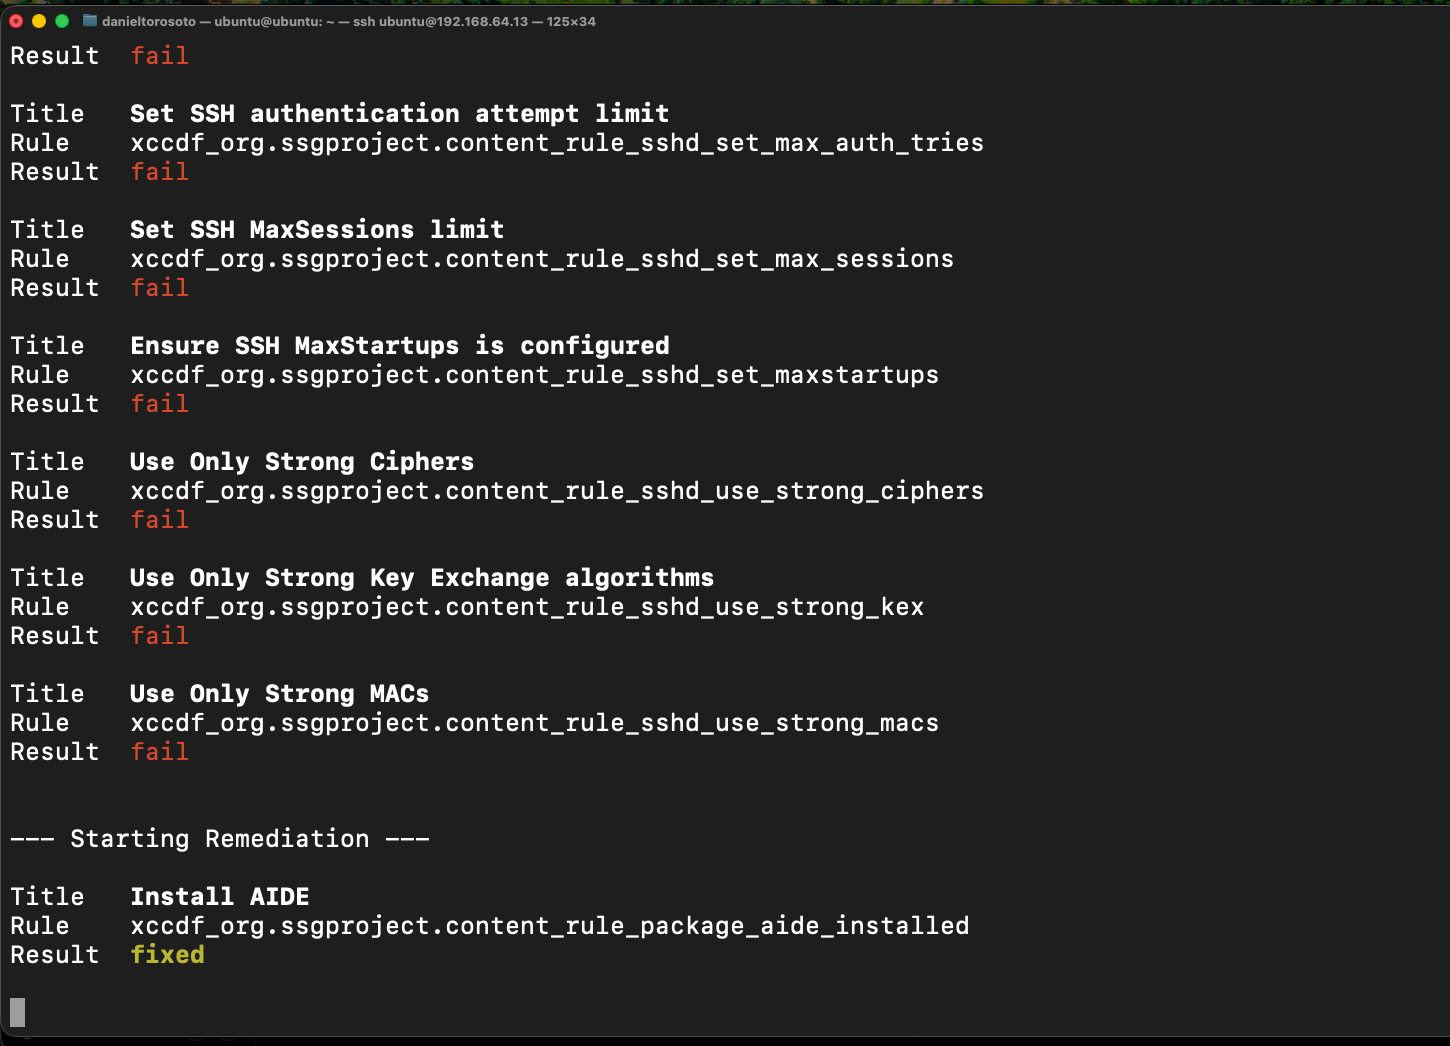
\includegraphics[width=0.85\textwidth]{../img/running_remediation.png}
  \caption{Ejecución de las remediaciones automáticas en curso.}
  \label{fig:remediacion}
\end{figure}

\subsection{Fase 6: Escaneo final (post-remediación)}

Tras el reinicio, se ejecutó nuevamente el escaneo con los mismos parámetros para obtener el estado del sistema después de las remediaciones:

\begin{lstlisting}[style=bashstyle, caption={Escaneo final tras las remediaciones}]
SSG="$HOME/scap-security-guide-0.1.76/ssg-ubuntu2404-ds.xml"

sudo oscap xccdf eval \
  --profile xccdf_org.ssgproject.content_profile_cis_level1_server \
  --results /tmp/resultado-final.xml \
  --report /tmp/reporte-final.html \
  "$SSG"
\end{lstlisting}

\subsection{Fase 7: Transferencia de reportes al Mac anfitrión}

Los archivos generados por OpenSCAP pertenecen al usuario \texttt{root} al ser ejecutados con \texttt{sudo}. Se copiaron al directorio home del usuario \texttt{ubuntu} y luego se transfirieron al Mac mediante SCP:

\begin{lstlisting}[style=bashstyle, caption={Transferencia de reportes via SCP}]
# En la VM: cambiar propietario
sudo cp /tmp/reporte-inicial.html ~/
sudo cp /tmp/reporte-final.html ~/
sudo chown ubuntu:ubuntu ~/reporte-*.html

# Desde el Mac (IP de la VM: 192.168.64.13)
scp ubuntu@192.168.64.13:~/reporte-inicial.html ~/Desktop/
scp ubuntu@192.168.64.13:~/reporte-final.html ~/Desktop/
\end{lstlisting}

% ============================================================
%  4. RESULTADOS
% ============================================================
\section{Resultados}

\subsection{Comparación de puntuación antes y después}

La evaluación con OpenSCAP asigna una puntuación porcentual al sistema en función de la proporción de controles aprobados sobre el total de controles evaluables. El Cuadro~\ref{tab:resultados} resume los resultados obtenidos en ambas evaluaciones.

\begin{table}[H]
\centering
\caption{Comparación de resultados del escaneo OpenSCAP (perfil CIS Level 1 Server)}
\label{tab:resultados}
\begin{tabular}{lcc}
\toprule
\textbf{Métrica} & \textbf{Escaneo inicial} & \textbf{Escaneo final} \\
\midrule
Puntuación total      & 65.56\%  & 90.25\%  \\
Reglas evaluadas      & 306      & 303      \\
Controles aprobados (pass)   & 171      & 288      \\
Controles fallidos (fail)    & 125      & 8        \\
No comprobados (notchecked)  & 10       & 7        \\
No aplicables (notapplicable)& 50       & 53       \\
\bottomrule
\end{tabular}
\end{table}

\subsection{Análisis de la mejora}

El sistema pasó de una puntuación de \textbf{65.56\%} en la evaluación inicial a \textbf{90.25\%} tras las remediaciones automáticas, lo que representa una mejora de \textbf{24.69 puntos porcentuales}. En términos absolutos, el número de controles aprobados aumentó de 171 a 288 (+117 controles), mientras que los controles fallidos se redujeron drásticamente de 125 a 8 (reducción del 93.6\%).

Los 8 controles que permanecieron en estado \textit{fail} tras las remediaciones corresponden típicamente a configuraciones que OpenSCAP no puede corregir de forma automatizada sin riesgo de interrumpir la operatividad del sistema, tales como:

\begin{itemize}
  \item Particionamiento de disco con puntos de montaje separados para \texttt{/tmp}, \texttt{/var}, \texttt{/home} (requiere reparticionado, no remediable en caliente).
  \item Configuraciones que dependen del entorno específico de despliegue.
  \item Controles que requieren intervención manual o reinicio adicional.
\end{itemize}

Esta puntuación final del 90.25\% posiciona al sistema en un nivel de cumplimiento alto con respecto al benchmark CIS Level 1, superando el umbral habitual de referencia del 80\% utilizado en muchas organizaciones.

\subsection{Controles más relevantes remediados}

Entre los controles CIS Level 1 que pasaron de \textit{fail} a \textit{pass} tras la remediación destacan:

\begin{itemize}
  \item \textbf{Configuración de SSH:} deshabilitación del acceso root directo (\texttt{PermitRootLogin no}), tiempo máximo de sesión inactiva, protocolo SSH2 obligatorio.
  \item \textbf{Auditoría del sistema:} instalación y configuración de \texttt{auditd} con reglas para monitorizar accesos al sistema, cambios de privilegios y modificaciones de archivos sensibles.
  \item \textbf{Módulos del kernel:} deshabilitación de módulos innecesarios como \texttt{usb-storage}, \texttt{cramfs}, \texttt{freevxfs}, \texttt{jffs2}, \texttt{hfs}, \texttt{hfsplus}, \texttt{udf} y protocolos de red no utilizados.
  \item \textbf{Políticas de contraseñas:} longitud mínima, complejidad, historial y período de vigencia mediante \texttt{PAM} y \texttt{/etc/login.defs}.
  \item \textbf{Firewall:} activación y configuración básica de \texttt{ufw} con política de denegación por defecto.
  \item \textbf{Permisos de archivos:} corrección de permisos en \texttt{/etc/passwd}, \texttt{/etc/shadow}, \texttt{/etc/group} y otros archivos sensibles del sistema.
\end{itemize}

% ============================================================
%  5. CONCLUSIONES
% ============================================================
\section{Conclusiones}

El presente trabajo demostró la eficacia de OpenSCAP y la SCAP Security Guide como herramientas para automatizar el hardening de sistemas Linux. A partir de una instalación base de Ubuntu Server 24.04, se logró elevar la puntuación de cumplimiento con el perfil CIS Level 1 del 65.56\% al 90.25\%, reduciendo los controles fallidos en un 93.6\%.

El proceso puso de manifiesto varias conclusiones relevantes:

En primer lugar, la instalación predeterminada de Ubuntu Server 24.04 ya incorpora algunos controles de seguridad básicos (65.56\% de cumplimiento inicial), pero dista significativamente de los estándares CIS. Esto subraya la necesidad de un proceso de hardening explícito antes de poner un servidor en producción.

En segundo lugar, la automatización mediante OpenSCAP permite aplicar cientos de controles de forma coherente y reproducible en cuestión de minutos, eliminando el error humano inherente a la configuración manual. El modo \texttt{--remediate} resultó especialmente eficaz, corrigiendo 117 controles en una sola ejecución.

En tercer lugar, existe un límite a lo que la remediación automática puede lograr: los 8 controles restantes evidencian que ciertos aspectos del hardening —principalmente el particionamiento de disco— deben planificarse desde la instalación del sistema operativo, antes de que este entre en producción.

Finalmente, la metodología SCAP ofrece la ventaja de la trazabilidad: los reportes XML y HTML generados constituyen evidencia auditable del estado de seguridad del sistema en un momento dado, lo que facilita el cumplimiento normativo y la auditoría interna.

% ============================================================
%  6. REFERENCIAS
% ============================================================
\section{Referencias}

\begin{flushleft}
\setlength{\parindent}{0pt}
\setlength{\hangindent}{0.5in}

Center for Internet Security. (2024). \textit{CIS Benchmarks: Consensus-based configuration guidelines}. \url{https://www.cisecurity.org/cis-benchmarks}

\medskip

ComplianceAsCode. (2024). \textit{SCAP Security Guide v0.1.76} [Software]. GitHub. \url{https://github.com/ComplianceAsCode/content/releases/tag/v0.1.76}

\medskip

National Institute of Standards and Technology. (2011). \textit{The Technical Specification for the Security Content Automation Protocol (SCAP): SCAP Version 1.2} (NIST Special Publication 800-126 Rev. 2). U.S. Department of Commerce. \url{https://doi.org/10.6028/NIST.SP.800-126r2}

\medskip

OpenSCAP. (2024). \textit{OpenSCAP: Open-source security compliance solution}. \url{https://www.open-scap.org}

\medskip

Canonical Ltd. (2024). \textit{Ubuntu Server 24.04 LTS (Noble Numbat) release notes}. \url{https://discourse.ubuntu.com/t/noble-numbat-release-notes/39890}

\medskip

Red Hat, Inc. (2024). \textit{Security hardening with OpenSCAP: Red Hat Enterprise Linux security guide}. \url{https://access.redhat.com/documentation/en-us/red_hat_enterprise_linux}

\end{flushleft}

% ============================================================
%  7. ANEXOS
% ============================================================
\section*{Anexos}
\addcontentsline{toc}{section}{Anexos}

\subsection*{Anexo A: Reporte HTML inicial}

El reporte generado por OpenSCAP tras el escaneo inicial (\texttt{reporte-inicial.html}) se incluye en la carpeta \texttt{resultados/} del repositorio del proyecto. Este reporte muestra el estado de cada uno de los 306 controles evaluados, con la siguiente distribución: 171 aprobados, 125 fallidos, 10 no comprobados y 50 no aplicables. La puntuación obtenida fue de \textbf{65.56\%}.

Para visualizar el reporte abrir el archivo con cualquier navegador web moderno. El archivo está autocontenido e incluye todo el JavaScript y CSS necesario para la visualización interactiva.

\subsection*{Anexo B: Reporte HTML final}

El reporte generado tras las remediaciones y el escaneo final (\texttt{reporte-final.html}) refleja la mejora obtenida: 288 controles aprobados, 8 fallidos, 7 no comprobados y 53 no aplicables sobre 303 controles evaluados. La puntuación final fue de \textbf{90.25\%}.

Ambos reportes se encuentran en el directorio \texttt{resultados/} del repositorio de la actividad.

\subsection*{Anexo C: Resumen de comandos ejecutados}

Los comandos completos ejecutados durante la actividad, incluyendo las salidas relevantes del terminal, se documentan en el archivo \texttt{commands.md} del repositorio.

\end{document}
